With the \tB{\emph{generative} approach we create a joint model of the form $\prob{y,\bm{x}}$, and
then to condition on $\bm{x}$, thereby deriving $\prob{y|\bm{x}}$}.\\
Alternatively, \tB{fitting directly a model of the form $\prob{y|\bm{x}}$ is a \emph{
discriminative} approach}.

\begin{itemize}
    \item \emph{Easy to fit}: generative classifiers is usually very easy
    \item \emph{Fit classes separately?}: in a generative classifier we estimate the parameters 
        of each class conditional density independently
    \item \emph{Handle missing features easily?}: in a generative classifier there is a natural way
        to handle missing data: $\prob{\bm{x}_{i},r_{i}|\bm{\theta},\bm{\phi}} = \prob{r_{i}|\bm{
        x}_{i},\bm{\phi}}\prob{\bm{x}_{i}|\bm{\theta}}$ where $\bm{\phi}$ are the parameters
        controlling whether the item is observed or not. Missing completely at random (MCAR): $\prob{
        r_{i}|\bm{x}_{i},\bm{\phi}} = \prob{r_{i}|\bm{x}^{0}_{i}|\bm{\phi}}$, missing at random 
        (MAR): $\prob{r_{i}|\bm{x}_{i},\bm{\phi}} = \prob{r_{i}|\bm{x}^{0}_{i},\bm{\phi}}$
    \item \emph{Can handle unlabeled training data?}: Fairly easy in using generative models
    \item \emph{Symmetric in inputs and outputs?}: We can run a generative model "backward" and 
        infer probable inputs given the output by computing $\prob{\bm{x}|y}$
    \item \emph{Can handle feature preprocessing?}: discriminative methods allow to preprocess the
        input in arbitrary ways, by replacing $\bm{x}$ with $\phi(\bm{x})$
    \item \emph{Well-calibrated probabilities?}: discriminative models are usually better calibrated
        in terms of their probability estimates.
\end{itemize}


\section{Classification}
% Naive Bayes Classifiers
\subsection{Naive Bayes classifiers}
\paragraph{Purpose}
\tR{Classifying vectors of discrete-valuated features $x\in\left\{i
\right\}_{1\leq i \leq K}^{D}$}, where $K$ is the number of values for
each feature, and $D$ the number of features.

\paragraph{Assumptions}
\begin{itemize}
    \item \tB{Features are conditionally independent given the class 
        label}
\end{itemize}

\paragraph{Theory}
As a \emph{generative} model, meaning of the form:
$\prob{y=c|\bm{x}, \bm{\theta}} \propto \prob{\bm{x}|y=c,\bm{\theta}}
\prob{y=c|\bm{\theta}}$. The key of such models is the possibility
to specify a suitable form for the class-conditional density 
$\prob{\bm{x}|y=c, \bm{\theta}}$ which definees what kind of data we 
expect to see in each class. And with the independence assumption we 
have:
\begin{center}
    \tB{$\prob{\bm{x}|y=c, \bm{\theta}} = \prd{j=1}{D}\prob{x_{j}|y=c,\bm{\theta}_{jc}}$}
\end{center}
with all $\prob{x_{j}|y=c,\bm{\theta}_{jc}}$ being able to 
follow a \textit{normal}, \textit{bernoulli} or \textit{multinoulli} 
distribution.\\
\uB{Training a NBC consists in computing the MLE or the MAP estimate for 
the parameters.}\\
For a single observation
$\prob{x_{i}, y_{i}|\bm{\theta}} = \prob{y_{i}|\bm{\pi}}\prd{j}{}\prob{x_{ij}|\bm{\theta}_{j}} = 
\prd{c}{}\pi_{c}^{\mathbbm{1}(y_{i}=c)}\prd{j}{}\prd{c}{}\prob{x_{ij}|
\theta_{jc}}^{\mathbbm{1}(y_{i}=c)}
$\\ 
Hence the \tB{\emph{log-likelihooh}:
$\log\left(\mathcal{D}|\theta\right) = \su{c=1}{C}N_{c}\log(\pi_{c}) + 
\su{j=1}{D}\su{c=1}{C}\su{i:y_{i}=c}{}\log\left(\prob{x_{ij}|
\bm{\theta}_{jc}}\right)$}\\
By optimizing the above equation we are able to find the $\left(\theta_{jc}\right)_{1\leq j \leq D,~ 1\leq c\leq C}$ and we can then use them to
predict the output of an observation $\bm{x}$ as: $\prob{y=c|\bm{x},\mathcal{D}} \propto \prob{y=c|\mathcal{D}}\prd{j=1}{D}\prob{x_{j}|y=c,\mathcal{D}}$

\paragraph{Strengths}
\begin{itemize}
    \item Simple model, for $C$ classes and $D$ features, and hence \tB{relatively immune to 
        overfitting}
\end{itemize}

\paragraph{Weaknesses}
\begin{itemize}
    \item \uB{Unaccuracy} because of the strong independence assumption
\end{itemize}

\paragraph{Relationships with other methods}
\tB{Logistic Regression}: for discrete inputs 
\emph{Naive Bayesian Classifiers} form a 
generative-discriminant pair with \emph{Multinomial Logistic
Regression}: \uB{each NBC can be considered a way of fitting a
probability model that optimizes the joint likelihood 
$\prob{C, \bm{x}}$, while Multinomial Logistic Regression fits the same 
probability to optimize the conditional $\prob{C|\bm{x}}$}

\paragraph{Examples of application}
\begin{itemize}
    \item Classifying documents using bag of words
    \item Determining the gender of a person, based on measured features 
\end{itemize}


% Linear/Quadratic Discriminant Analysis
\subsection{Linear/Quadratic Discriminant Analysis}
\uB{It consists in defining the class conditional densities in a 
generative classifier}: $\prob{\bm{x}|y=c,\bm{\theta}} = \mathcal{N}
\left(\bm{x}, \bm{\mu}_{c},\bm{\Sigma}_{c}\right)$\\
As for a generative classifier we have the following equation: 
\begin{center}
    $\prob{y=c|\bm{x},\bm{\theta}} = \dfrac{\overbrace{\prob{\bm{x}|y=c,
        \bm{\theta}}}^{\text{\emph{class-conditional density}}}
        \overbrace{\prob{y=c|\bm{\theta}}}^{\text{\emph{class prior}}}}{
    \su{c'}{}\prob{y=c'|\bm{\theta}} \prob{\bm{x}|y=c',\bm{\theta}}}$
\end{center}
\paragraph{Purpose of Quadratic Discriminant Analysis}
\begin{center}
    $\prob{y=c|\bm{x},\bm{\theta}} = \dfrac{|2\pi\Sigma_{c}|^{
    -\frac{1}{2}}\exp\left(-\frac{1}{2}[\bm{x}-\bm{\mu}_{c}]^{T}\Sigma_{
    c}^{-1}[\bm{x}-\bm{\mu}_{c}]\right)\pi_{c}}{\su{c'}{}|2\pi\Sigma_{
    c'}|^{-\frac{1}{2}}\exp\left(-\frac{1}{2}[\bm{x}-\bm{\mu}_{c'}]^{T}
    \Sigma_{c'}^{-1}[\bm{x}-\bm{\mu}_{c'}]\right)\pi_{c'}}$
\end{center}
\tB{The threshold of this results will be a quadratic function of 
$\bm{x}$.}

\paragraph{Purpose of Linear Discriminant Analysis}
Same equation than above but this time, \tB{$\forall c\in \inter{1}{C} 
\Sigma_{c} = \Sigma$}, \tB{then quadratic term $\bm{x}^{T}\Sigma^{-1}
\bm{x}$ will cancel out from numerator and denominator}.
Then by considering the above cancellation and the fact that 
evidence is considered as a constant, we have:
\tB{
\begin{align*}
    \prob{y=c|\bm{x},\bm{\theta}} & \propto \exp\left(\log(\pi_{c})+\bm{
        \mu}_{c}^{T}\Sigma^{-1}\bm{x}\bm{\mu}_{c}\right)\\
    &= \exp\left(\bm{\beta}_{c}^{T}\bm{x} + \gamma_{c}\right)
    \end{align*}
}
Note also that we have exactly: \tR{$\prob{y=c|\bm{x},\bm{\theta}} =
\dfrac{e^{\bm{\beta}_{c}^{T}\bm{x} + \gamma_{c}}}{\su{c'}{}e^{\bm{\beta
}_{c'}^{T}\bm{x} + \gamma_{c'}}} = S(\bm{\eta})_{c}$}. With $\eta=\left(
\bm{\beta}_{c}\bm{x} +\gamma_{c}\right)_{1\leq c\leq C}$
We recognize the \emph{softmax} function.

\paragraph{Assumptions}
\begin{itemize}
    \item Independent \tB{variables are normal for each level} of the
        grouping variable.
    \item \tB{Homoscedasticity} for LDA: variances \uB{among group} 
        variables are the same across levels of predictors.
    \item \uB{Independence of the observations}.
\end{itemize}


\paragraph{Theory}
\paragraph{Strengths}
\paragraph{Weaknesses}
\begin{itemize}
    \item Multicollinearity: predictive power can decrease with an 
        increased correlation between predictor variables.
\end{itemize}

\paragraph{Relationships with other methods}
\paragraph{Examples of application}


\subsection{Logistic Regression}
\paragraph{Purpose}
With the generative approach we create a joint model of the form $\prob{y,\bm{x}}$, and
then to condition on $\bm{x}$, thereby deriving $\prob{y|bm{x}}$, it is the \emph{
generative} approach.\\
Alternatively, fitting directly a model of the form $\prob{y|\bm{x}}$ is a \emph{
discriminative} approach.
\paragraph{Assumptions}
\begin{itemize}
    \item Independence
\end{itemize}

\paragraph{Theory}
The data distribution is modelled by : 
\fr{$\prob{y|\bm{x}} = \text{\emph{Bernoulli}} \left(y|\sigma\left(\bm{w}^{T}\bm{x}
\right)\right)$}\\
With $\sigma$ being the \emph{sigmoid} function, such that 
$\sigma = \begin{cases}
    \mathbb{R} \longrightarrow [0, 1]\\ 
    x \mapsto \dfrac{e^{x}}{1 + e^{x}}
\end{cases}
$
\subparagraph{Maximum Likelihood Estimator}
\begin{align*}
    \text{\emph{NLL}}(\bm{w})
    &= -\su{i=1}{N}\log\left(\hat{y}_{i}^{\mathbbm{1}_{\{y_{i} = 1\}}}\left[1 -
    \hat{y}_{i}\right]^{\mathbbm{1}_{\{y_{i}=0\}}}\right)\\ 
    &= -\su{i=1}{N}y_{i}\log\left(\hat{y}_{i}\right) + \left[1 -y_{i}\right]\log
    \left(1 -\hat{y}_{i}\right)
\end{align*}
This called \textit{cross-entropy}


\paragraph{Strengths}
\paragraph{Weaknesses}
\paragraph{Relationships with other methods}
\paragraph{Examples of application}

\subsection{Fisher's Linear Discriminant Analysis (FLDA)}
\paragraph{Purpose}
An alternative way to the above discriminant analysis is to reduce the dimensionality
of the features $\bm{x}\in\mathbb{R}^{D}$ and then fit a Multivariate Normal to the 
resulting low-dimensional features $\bm{z}\in \mathbb{R}^{L}$.\\
\emph{PCA} would not be a good idea because it is unsupervised and the low-dimensional
resulting features would not be optimal for the classification problem.\\
A better option would be to \uB{find a matrix $\bm{W}$ such that the low-dimensional 
data can be classified as well as possible using a Gaussian class-conditional density 
model}, this is the \emph{FLDA}.
\paragraph{Assumptions}
\begin{itemize}
    \item Gaussian class-conditional: reasonable since we are computing linear 
        combination of potentially non-Gaussian features.
\end{itemize}

\paragraph{Theory}
For $2$ classes
Let us define 
$\begin{cases}
    \mu_{1} = \frac{1}{N_{1}}\su{i:y_{i}=1}{}\bm{x}_{i}\\
    \mu_{2} = \frac{1}{N_{2}}\su{i:y_{i}=2}{}\bm{x}_{i}
\end{cases}$,
and $m_{k} = \bm{w}^{T}\bm{\mu}_{k}$ being the projection of each mean onto the line
$\bm{w}$. Also let $z_{i}=\bm{w}^{T}\bm{x}_{i}$ be the projection of the data onto the 
line $\bm{w}$.\\
The goal is to find $\bm{w}$ such that we maximize the distance between the means,
$m_{1} - m_{2}$, while also ensuring the projected clusters are "tight":
\begin{center}
    $\bm{J}(\bm{w}) = \dfrac{(m_{f} - m_{1})^{2}}{s_{1}^{2} + s_{2}^{2}}
    = \dfrac{\bm{w}^{T}\bm{S}_{B}\bm{w}}{\bm{w}^{T}\bm{S}_{W}\bm{w}}$
\end{center}
with the \emph{between-class scatter matrix}: $\bm{S}_{B} = \left(\mu_{2} - \mu_{1}
\right)\left(\mu_{2} - \mu_{1}\right)^{T}$ and \emph{within-class scatter matrix}:
$
\su{i:y_{i}=1}{}\left(\bm{x}_{i} - \bm{\mu}_{1}\right) \left(\bm{x}_{i} - 
\bm{\mu}_{1}\right)^{T} + \su{i:y_{i}=2}{}\left(\bm{x}_{i} - \bm{\mu}_{2}\right)\left(
\bm{x}_{i} - \bm{\mu}_{2}\right)^{T}
$


\paragraph{Strengths}
\begin{itemize}
    \item Classification in taking in account the response label.
\end{itemize}

\paragraph{Weaknesses}
\begin{itemize}
    \item FLDA is restricted to using $L\leq C-1$ dimensions, regardless of $D$.
\end{itemize}

\paragraph{Relationships with other methods}
\begin{itemize}
    \item Linear Discriminant Analysis
    \item PCA
\end{itemize}

\paragraph{Examples of application}
\begin{itemize}
    \item Speech recognition
\end{itemize}


%\subsection{Logistic Regression}
%\paragraph{Purpose}
%\paragraph{Assumptions}
%\paragraph{Theory}
%\paragraph{Strengths}
%\paragraph{Weaknesses}
%\paragraph{Relationships with other methods}
%\paragraph{Examples of application}


\section{Regression}
\subsection{Linear Regression}
\paragraph{Purpose}
\paragraph{Assumptions}
\paragraph{Theory}
\subparagraph{General}
It is a model for which the data distribution (likelihood) is described 
by:
\tR{\begin{center}
    $\prob{y|\bm{x},\bm{\theta}} = \mathcal{N}\left(y|\bm{w}^{T}\phi(
    \bm{x}), \sigma^{2}\right)$
\end{center}}
with $\phi$ that can be a non-linear function, in this case we talk about
\emph{basis function expansion}.\\
To estimate the parameters we can use the \emph{maximum likelihood 
estimation}: \tB{$\hat{\theta} \triangleq \argmax_{\theta} \log\left(
\prob{\mathcal{D}|\bm{\theta}}\right)$}.\\
For computational purpose it is better to consider the minimization of 
the \textit{Negative Log Likelihood} (NLL):
\begin{align*}
    \text{\emph{NLL}}(\theta) &\triangleq -\log\left(p\left(\mathcal{D}|
    \theta\right)\right)\\
                              &=-\su{i=1}{n}\log\left(\prob{y_{i}|
                                      \bm{x}_{i},\bm{\theta}}\right)\\
                              &=-\su{i=1}{n}\log\left(\left[\dfrac{1}{
                              2\pi\sigma^{2}}\right]^{\frac{1}{2}}\exp
                              \left(-\dfrac{1}{2\sigma^{2}}\left[y_{i}
                                      - \bm{w}^{T} \bm{x}_{i}\right]^{2}
                              \right)\right)\\
                              &= \dfrac{n}{2}\log\left(2\pi\sigma^{2}
                              \right) + \dfrac{1}{2\sigma^{2}}\su{i=1}{
                              n}\left(y_{i} - \bm{w}^{T}\bm{x}_{i}
                              \right)^{2}\\
                              &= \dfrac{n}{2}\log\left(2\pi\sigma^{2}
                              \right) + \dfrac{1}{2\sigma^{2}}\text{
                              \emph{RSS}}(\bm{w})\\
                              &= \dfrac{n}{2}\log\left(2\pi\sigma^{2}
                          \right) + \dfrac{1}{2\sigma^{2}}\norm{\epsilon
                          }_{2}^{2}
\end{align*}
As the \emph{MLE} for $\bm{w}$ is the one minimizing the \emph{RSS} then
this method is known as \emph{least square}.

\subparagraph{Derivation of the MLE}
it is better to use a matrix-vector representation.\\
$\text{\emph{NLL}}(\bm{w}) = \dfrac{1}{2}\left(y-\bm{X}\bm{w}\right)^{T}\left(y-\bm{X}
\bm{w}\right) = \dfrac{1}{2}\bm{w}^{T}\left(\bm{X}^{T}\bm{X}\right)\bm{w} - \bm{w}^{T}
\left(\bm{X}^{T}y\right)$ Note that $\bm{X}^{T}\bm{X}$ is the \emph{sum of squares 
matrix}. Then \textbf{gradient}, $g(\bm{w}) = \bm{X}^{T}\bm{X}\bm{w} - \bm{X}^{T}\bm{y}$
that we have to equate to zero to get $\bm{X}^{T}\bm{X}\bm{w} = \bm{X}^{T}\bm{y}$ to 
conclude that:
\begin{center}
    \fr{$\hat{\bm{w}}_{OLS} = \left(\bm{X}^{T}\bm{X}\right)^{-1}\bm{X}^{T}\bm{y}$}
\end{center}

\subparagraph{Robust Linear Regression}
It is very common to model the noise in regression models using a \emph{Gaussian 
distribution}, meaning \tR{$\epsilon_{i} = y_{i} - \bm{w}^{T}\bm{x}_{i} \hookrightarrow 
\mathcal{0, \sigma^{2}}$}. One way to achieve \emph{robustness} against \emph{outliers}
is to replace the Gaussian distribution for the response variable with a distribution 
having \textbf{heavy tails}.

\begin{center}
    \begin{tabular}{|*{3}{c|}}
    \hline
    \textbf{Likelihood} & \textbf{Prior} & \textbf{Name}\\
    \hline
    Gaussian & Uniform & \emph{Least Squares}\\
    \hline
    Gaussian & Gaussian & \emph{Ridge}\\
    \hline
    Gaussian & Laplace & \emph{Lasso}\\
    \hline
    \end{tabular}
\end{center}

\subparagraph{Ridge}
encourages parameters to be small by using a zero-mean Gaussian prior: $\prob{\bm{w}} = 
\prd{j=1}{D} \mathcal{N}\left(\omega_{j}|0, \tau^{2}\right)$, where $\frac{1}{\tau^{2}}$
controls the strength of the prior.\\
The corresponding \tB{\emph{MAP}} estimation problem becomes:
\tB{$\argmax_{\bm{w}}\su{i=1}{n}\log\left(\mathcal{N}\left(y_{i}|\omega_{0} + \bm{w}^{T}
\bm{x}_{i}, \sigma^{2}\right)\right) + \su{j=1}{D}\log\left(\mathcal{N}\left(\omega_{j}
|0,\tau^{2} \right)\right)$}. After some calculus and with where $\lambda \triangleq 
\dfrac{\sigma^{2}}{\tau^{2}}$ we deduce that:
\begin{center}
    \fr{$
        \hat{\bm{w}}_{\text{\emph{Ridge}}} = \left(\lambda\bm{I}_{D} + \bm{X}^{T}\bm{X}
        \right)^{-1}\bm{X}\bm{y}
    $}
\end{center}
Advantages of Ridge regression on OLS regression:
\begin{itemize}
    \item $\left(\lambda\bm{I}_{D}+\bm{X}^{T}\bm{X}\right)$ is much better conditioned, 
        and hence more likely to be invertible, than $\bm{X}^{T}\bm{X}$ at least for 
        suitable large $\lambda$
    \item if we follow a \emph{Singular Value Decomposition} $\bm{X} = \bm{U}\bm{S}
        \bm{V}^{T}$ we find 
        that $\hat{\bm{y}} = \bm{X}\hat{\bm{w}}_{\text{\emph{Ridge}}} = \su{j=1}{D}
        \bm{u}_{j}\dfrac{\sigma_{j}^{2}}{\sigma_{j}^{2} + \lambda}\bm{u}_{j}^{T}\bm{y}$
        with $\left(\sigma_{j}\right)_{1\leq j \leq D}$ the singular value of $\bm{X}$
        whereas for OLS we have $\hat{\bm{y}} = \bm{X}\hat{\bm{w}}_{\text{\emph{OLS}}} 
        = \su{j=1}{D} \bm{u}_{j}\bm{u}_{j}^{T}\bm{y}$. Meaning that with Ridge if 
        $\sigma_{j}^{2}$ is small compared to $\lambda$ then direction $\bm{u}_{j}$
        will not have much effect on the prediction. In term of predictive accuracy
        \emph{Ridge} regression is more interesting than \emph{PCA} regression.
\end{itemize}

\paragraph{Strengths}
\begin{itemize}
    \item Simple
    \item Customizable to achieve robustness
\end{itemize}

\paragraph{Weaknesses}
\begin{itemize}
    \item Not very powerful for non-linear data

\end{itemize}

\paragraph{Relationships with other methods}
\begin{itemize}
    \item Ridge Regression has similitude with PCA
\end{itemize}

\paragraph{Examples of application}



\section{Classification and Regression}
\subsection{Mutlt-task}
\paragraph{Purpose}
To fit many related classification or regression models at the same time, as it is often reasonable
to assume the input-output mappings is similar across these different models.

\paragraph{Assumptions}
\begin{itemize}
    \item Input/Output mapping
\end{itemize}

\paragraph{Theory}
\subparagraph{Hierarchical Bayes for multi-task learning}
Let consider $y_{ij}$ the response of the $i^{th}$ item in group $j$ with $(i,j)\in\inter{1}{N_{j}}
\times\inter{1}{J}$.\\
Although some groups may have lot of data, there is often a long tail where the majority of groups
have little data. Thus we can't reliably fit each model separately but we don't want to use the
same model for all the groups. As a compromise, \tB{we can fit a separate model for each group but
encourage the model parameters to be similar across the groups}. More precisely:
\begin{center}
    $\begin{cases}
        \E{y_{ij}|\bm{x}_{ij}} = g(\bm{x}_{ij}^{T}\bm{\beta}_{j}) \\
        \bm{\beta}_{j} \hookrightarrow \mathcal{N}\left(\bm{\beta}_{*}, \sigma_{j}^{2}\bm{I}\right)\\
        \bm{\beta}_{*} \hookrightarrow \mathcal{N}\left(\bm{\mu}, \sigma_{*}^{2}\bm{I}\right)
    \end{cases}$
\end{center}
$\bm{\beta}_{j}$ is a coefficient vector associated with the group $j$.\\
Also \uB{groups with small sample size borrow statistical strength from the groups with larger sample
size because the $\bm{\beta}_{j}$'s are correlated via the latent common parents $\bm{\beta}_{*}$}.\\
The term $\sigma_{j}^{2}$ controls how much group $j$ depends on the common parents and the 
$\sigma_{*}^{2}$ term controls the strength of the overall prior.
\paragraph{Strengths}
\begin{itemize}
    \item Performance improvement
\end{itemize}

\paragraph{Weaknesses}
\paragraph{Relationships with other methods}
\paragraph{Examples of application}
\begin{itemize}
    \item Determine the test scores for a given student in a given school without using as many 
        models as school count
    \item Personal spam filtering: 
\end{itemize}


\subsection{Mixture models}
\paragraph{Purpose}
It is the \tR{simplest form of \emph{Latent Variable Models (LVMs)} is when $z_{i}\in
\inter{1}{K}$}.\\
Two mains application of mixture models:
\begin{itemize}
    \item use them as \emph{black-box} density model, $p(\bm{x}_{i})$, useful for \tB{data
        compression, outlier detection and creating generative classifiers}
    \item use for \tB{clustering}
\end{itemize}

\paragraph{Assumptions}
\paragraph{Theory}
We use a \tB{discrete prior $p(z_{i}) = \text{\emph{Cat}}(\bm{\pi})$} and the likelihood
$p(\bm{x}_{i}|z_{i} = k)$, finally the \textbf{mixture model} is :
\begin{center}
    \tR{$\prob{\bm{x}_{i}|\bm{\theta}} = \su{k=1}{K}\pi_{k}\prob{\bm{x}_{i}|z_{i}=k,
    \bm{\theta}} = \su{k=1}{K}\pi_{k}\mathbb{P}_{k}\left(\bm{x}_{i}|\bm{\theta}\right)$}
\end{center}
where \uB{$\mathbb{P}_{k}$ is the $k$'th \emph{base distribution}}.
\subparagraph{Mixtures of Gaussian}
Each base distribution in the mixture is a multivariate Gaussian with mean $\mu_{k}$ 
and covariance matrix $\bm{\Sigma}_{k}$:
\tB{$\prob{\bm{x}_{i}|\bm{\theta}}=\su{k=1}{K}\pi_{k}\mathcal{N}\left(\bm{x}_{i}|\bm{\mu}_{k},
    \bm{\Sigma_{k}}\right)$}\\
Given a sufficiently large number of mixture components a \tR{Gaussian Mixture Models
(GMMs) can be used to approximate any density defined on $\mathbb{R}^{D}$}.
\subparagraph{Mixtures of multinoullis}
can be used to define density models on data consisting of a \emph{D}-dimensional bit
vectors: \tB{$\prob{\bm{x}_{i}|z_{i}=k,\bm{\theta}} = \prd{j=1}{D}\text{\emph{Ber}}(x_{ij}|
\mu_{jk})=\prd{j=1}{D}\mu_{jk}^{x_{ij}}(1-\mu_{jk})^{1-x_{ij}}$}\\
where \uB{$\mu_{jk}$ is the probability that bit $j$ turns on in cluster $k$}.
\subparagraph{Mixture models for clustering}
We first fit the mixture model an then compute \uB{$\prob{z_{i}=k|\bm{x}_{i},\bm{\theta}}$ 
representing the posterior probability that point $i$ belongs to cluster $k$}.\\
This known as the \emph{responsibility} of cluster $k$ for point $i$ and can be computed using 
Bayes:
\begin{center}
    \fr{$r_{ik} \triangleq \prob{z_{i}=k|\bm{x}_{i},\bm{\theta}} = \dfrac{\prob{z_{i}=k|\bm{\theta}}
    \prob{\bm{x}_{i}|z_{i}=k,\bm{\theta}}}{\su{k'=1}{K}\prob{z_{i}=k'|\bm{\theta}}\prob{\bm{x}_{i}|
    z_{i}=k',\bm{\theta}}}$}
\end{center}

\subparagraph{Mixture of experts}
are build from a discriminative perspective, they relies on the idea that a good
model can be achieved in \tB{using multiple different linear method each applying to a different part
of the input space}.\\
We can model this by allowing the mixing weights and the mixture densities to be
input-dependent: 
\begin{center}
    $\begin{cases}
        \prob{y_{i}|\bm{x}_{i},z_{i}=k,\bm{\theta}} = \mathcal{N}(y_{i}|\bm{w}_{k}^{T}
        \bm{x}_{i},\sigma_{k}^{2}) \\
        \prob{z_{i}|\bm{x}_{i},\bm{\theta}} = \text{\emph{Cat}}(z_{i}|S(\bm{V}^{T}
        \bm{x}_{i}))
    \end{cases}$
\end{center}
Useful in solving inverse problems, the ones in which we have to invert a many-to-one
mapping, for example in robotics where the location of the end effector (hand) $\bm{y}$
is uniquely determined by the joint angles of the motors, $\bm{x}$.

The overall posterior is then
\begin{center}
    \fr{$\prob{y_{i}|\bm{x}_{i},\bm{\theta}} = \su{k}{}\prob{z_{i}=k|\bm{x}_{i},z_{i}=k
    ,\bm{\theta}}$}
\end{center}
 This model can be easily generalized to discrete data using the exponential family.
The model is usually fit with \emph{Expectation-Maximization} technique.
\paragraph{Strengths}

\paragraph{Weaknesses}
\begin{itemize}
    \item Use of a single latent variable to generate the observation
\end{itemize}

\paragraph{Relationships with other methods}
\paragraph{Examples of application}


\subsection{ARD: Automatic Relevance Determination}
\paragraph{Purpose}
To get \tB{greater sparsity} 
\paragraph{Assumptions}
\paragraph{Theory} 
Relying on \tB{empirical Bayes, whereby we integrate out $\bm{w}$ and maximize the 
marginal likelihood} $\tau$.
\subparagraph{Linear Regression}
Let's consider weight precisions by $\alpha_{j}=\frac{1}{\tau_{j}^{2}}$ and the 
measurement precision by $\beta=\frac{1}{\sigma^{2}}$:
\begin{center}
    $\begin{cases}
        \prob{y|\bm{x},\bm{w},\beta} = \mathcal{N}\left(y|\bm{w}^{T}\bm{x},\frac{1}{
            \beta}\right) \\
            \prob{\bm{w}} = \mathcal{N}(\bm{w}|0,\bm{A}^{-1})
    \end{cases}$
\end{center}
where $\bm{A}=\text{\emph{diag}}(\bm{\alpha})$
To regularize the problem we may put a conjugate prior on each precision $\alpha_{j}
\hookrightarrow \text{\emph{Gamma}}(a, b)$ and $\beta \hookrightarrow \text{\emph{
Gamma}}(c, d)$
When performing EB point estimation will use the improper prior $a=b=c=d=0$ which
results in \tB{maximal sparsity}.
\subparagraph{Sparsity}
If $\hat{\alpha}_{j} \approx 0$ we find $\hat{w}_{j}\approx \hat{w}^{mle}_{j}$ since
the Gaussian prior shrinking $w_{j}$ towards 0 has zero precision.\\
However if we find that \uB{$\hat{\alpha}_{j}\rightarrow\infty$ then the prior is very 
confident that $w_{j}=0$ and hence that feature $j$ is "irrelevant"}.
\subparagraph{Logistic Regression}
uses iteratively reweighted $l_{1}$ algorithm.

\paragraph{Strengths}
\begin{itemize}
    \item Resilient against uninformative features
\end{itemize}

\paragraph{Weaknesses}
\paragraph{Relationships with other methods}
\paragraph{Examples of application}



\subsection{Sparse coding}
\paragraph{Purpose}
Sparse priors for unsupervised learning, here we relax the constraint that $\bm{W}$
is orthogonal. 
\paragraph{Assumptions}
\paragraph{Theory}
\paragraph{Strengths}
\paragraph{Weaknesses}
\paragraph{Relationships with other methods}
\paragraph{Examples of application}

\subsection{Support Vector Machines (SVMs)}
\paragraph{Purpose}
The \tB{combination of the \emph{kernel trick} plus a modified loss function 
allowing \emph{sparsity}}, meaning that the prediction will only depend on a
subset of the training data called \emph{support vectors}. The overall 
process is known as a \emph{Support Vector Machine}.\\
Because of sparsity encoding in the loss function instead of in the prior, 
kernel encoding through a trick instead of being an explicit part of the 
model,\tB{SVMs do not provide probabilistic outputs}.
\subparagraph{SVMs for regression}
with \emph{kernalized ridge regression} the solution $\bm{w}$ depends on all 
the training inputs. We should then use a variant of \emph{Huber loss} 
function: the \tB{\textit{epsilon insensitive loss function}}: 
\begin{center}
    \fr{$L_{\epsilon}\left(y-\hat{y}\right) = 
    \begin{cases}
        0 & \Leftarrow \lvert y-\hat{y}\rvert < \epsilon \\
        \lvert y-\hat{y}\rvert -\epsilon &\Leftarrow \lvert y-\hat{y}\rvert 
            \geq \epsilon    
    \end{cases}$}
\end{center}
meaning that any point lying inside an $\epsilon\text{-\textbf{tube}}$ a
around the prediction is not penalized: $J=C\su{i=1}{n}L_{\epsilon}\left(
y_{i} - \hat{y}_{i}\right) + \frac{1}{2}\norm{\bm{w}}^{2}$, with $C=\frac{1}{
\lambda}$ is a \emph{regularization constant}.\\
It can be shown that \tB{optimal solution has the form $\hat{\bm{w}} = \su{i}{
}\alpha_{i} \bm{x}_{i}$, where $\alpha_{i}\geq 0$}. It turns out that \tB{
$\bm{\alpha}$ is sparse as we don't care about errors which are smaller than 
$\epsilon$. The $\bm{x}_{i}$ for which $\alpha_{i}>0$ are the \textbf{support 
vectors}}.\\
Then we have $\hat{y}(\bm{x}) = \hat{w}_{0} + \hat{\bm{w}}\bm{x}  = \hat{w}_{0}
+ \su{i}{}\alpha_{i}\bm{x}_{i}^{T}\bm{x} = \su{i}{}\alpha_{i}k(\bm{x},\bm{x}_{i})$

\subparagraph{Classification}
we consider now the \emph{hinge loss}:
\begin{center}
    \fr{$L_{hinge}(y,\eta) = \max\left(0, 1-y\eta\right) = \left(1-y\eta\right)_{+}$} 
\end{center}
where $\eta=f(\bm{x})$ is our 'confidence' in choosing label $y=1$ however it does not
need to have any probabilistic semantics.\\
The overall objective has the form $\min_{\bm{w}:w_{0}}\frac{1}{2}\norm{\bm{w}}^{2} +
C\su{i=1}{n}\left(1-y_{i}f(\bm{x}_{i})\right)_{+}$. Same principle as in regression, but
this time \tB{$\hat{y}(\bm{x}) = sgn\left(f(\bm{x})\right) = sgn\left(\hat{w}_{0} +
\hat{\bm{w}}^{T}\bm{x}\right)= sgn\left(\hat{w}_{0} + \su{i=1}{n}\alpha_{i}k(\bm{x}_{i}
,\bm{x})\right)$}
\subparagraph{The large margin principle}
our goal is to derive a \emph{discriminative function} $f(x)$ which will be linear in the feature
space implied by the choice of kernel. Hence: $\bm{x} = \bm{x}_{\perp} + 
r\frac{\bm{w}}{\norm{\bm{w}}}$ where $r$ is the distance of $\bm{x}$ from the decision boundary 
whose normal vector is $\bm{w}$, and $\bm{x}_{\perp}$ is the orthogonal projection of $\bm{x}$
onto this boundary. Hence $f(\bm{x}) = \bm{w}^{T}\bm{x} +w_{0} = \left(\bm{w}^{T}\bm{x}_{\perp}
+ w_{0}\right) + r\frac{\bm{w}^{T}\bm{w}}{\norm{\bm{w}}}$. As $f(\bm{x}_{\perp}) = 0$,
$\bm{w}^{T}\bm{x}_{\perp} +w_{0} = 0$ Hence $f(\bm{x}) = r\frac{\bm{w}^{T}\bm{w}}{\norm{\bm{w}}}$.
Finally \tB{$r = \frac{f(\bm{x})}{\norm{\bm{w}}}$, the distance that we would like to make as large 
as possible, in order to clearly separate the input}.
\subparagraph{Regularization parameter \emph{C}}
it \tB{controls the number of errors we are willing to tolerate on the training set}, it is chosen by
cross-validation, \uB{an efficient way to chose \emph{C} is to develop a path following algorithm in 
the spirit of \emph{ARS}}.

\paragraph{Assumptions}
\paragraph{Theory}
\paragraph{Strengths}
\begin{itemize}
    \item computational advantages over probabilistic model
    \item \tB{\emph{kernel trick} $\rightarrow$ prevent underfitting}: ensuring that the feature 
        vector is sufficiently rich that a linear classifier can separate
    \item \tB{\emph{sparsity} \& \emph{large margin principles} $\rightarrow$  prevent overfitting}: 
        ensure that we do not use all the basis functions

\end{itemize}

\paragraph{Weaknesses}
\begin{itemize}
    \item issues for multi-class classification due to the non-probabilistic 
        aspect of the model: \uB{output scores are not on a calibrate scale}
\end{itemize}

\paragraph{Relationships with other methods}
\paragraph{Examples of application}

\subsection{MODEL COMPARISON}
\paragraph{Comparison of discriminative kernel methods}
\begin{itemize}
    \item \emph{L1VM}: $l_{1}$-regularized vector machine
    \item \emph{L2VM}: $l_{2}$-regularized vector machine
    \item \emph{SVM}: Support Vector Machine
    \item \emph{RVM}: Relevance Vector Machine
    \item \emph{GP}: Gaussian Process
\end{itemize}
\begin{itemize}
    \item \emph{speed} $\rightarrow$ use RVM
    \item \emph{well-calibrated probabilistic outputs} $\rightarrow$ GP
\end{itemize}
the only circumstances under which using an SVM seems sensible is the structured output
case, where likelihood-based methods can be slow.


\subsection{Gaussian Processes}
\paragraph{Purpose}
It defines a prior over functions, which can be converted into a posterior over 
functions once we have seen some data.\\
They \tB{can be thought of as a Bayesian alternative to the kernel methods}.
In Python we can use the library \href{https://gpflow.github.io/GPflow/develop/index.html}{\emph{
GPflow}}
\paragraph{Assumptions}
\paragraph{Theory}
\subparagraph{Regression}
Let the prior on the regression function be GP denoted by:
\begin{center}
    \fr{$\begin{cases}
            f(\bm{x}) &\hookrightarrow \text{\emph{GP}}(m(\bm{x}), k(\bm{x},\bm{x}'))\\
            m(\bm{x}) &= \E{f(\bm{x})}\text{ \emph{the mean function}}\\
            k(\bm{x}, \bm{x}') &= \E{\left[f(\bm{x})-m(\bm{x})\right]^{T}\left[f(\bm{x}')-m(\bm{x}')
            \right]}\text{ \emph{kernel or covariance function}}
    \end{cases}$}
\end{center}
For any finite set of points, this process defines a joint Gaussian:
$\prob{\bm{f}|\bm{X}} = \mathcal{N}\left(\bm{f}[\bm{\mu},\bm{K}\right)$.\\
Where $\bm{K}$ is defined by $k_{ij}=k(\bm{x}_{i}, \bm{x}_{j})$ and $\bm{\mu}=\left(m(\bm{x}_{i})
\right)_{1\leq i\leq n}$\\
Let's consider the case where we predict using noise-free observation.
Suppose we observe a \tB{training observation set $\mathcal{D}=\left\{(\bm{x}_{i},f_{i})\right\}_{1
\leq i\leq n}$}, where $f_{i} = f(\bm{x}_{i})$ is the noise-free observation of the function 
evaluated at $\bm{x}_{i}$. Given a test set $\bm{X}_{*}$ of size $n_{*}\times D$ we want to predict
the function output $\bm{f}_{*}$.
\tB{The Gaussian Process will act as an \emph{interpolator} of the training data}.
\begin{center}
    \tB{$\begin{bmatrix}
        \bm{f}\\
        \bm{f}_{*}
    \end{bmatrix}
    \hookrightarrow\mathcal{N}\left(
        \begin{bmatrix}
            \bm{\mu}\\
            \bm{\mu}_{*}
        \end{bmatrix},
        \begin{bmatrix}
            \bm{K} & \bm{K}_{*}\\
            \bm{K}_{*}^{T} & \bm{K}_{**}
        \end{bmatrix}
    \right)$}
\end{center}
where $\bm{K}=k(\bm{X},\bm{X})$, $\bm{K}_{*}=k(\bm{X},\bm{X}_{*})$ and $\bm{K}_{**}=k(\bm{X}_{*},
\bm{X}_{*})$. By teh standard rules for conditioning Gaussians, the prosterior has the following 
form:
\fr{$\begin{cases}
    \prob{\bm{f}_{*}|\bm{X}_{*},\bm{X},\bm{f}} &= \mathcal{N}(\bm{f}_{*}|\bm{\mu}_{*},
    \bm{\Sigma}_{*})\\
    \bm{\mu}_{*} &= \bm{\mu}(\bm{X}_{*}) + \bm{K}_{*}^{T}\bm{K}^{-1}\left(\bm{f}-\bm{\mu}(\bm{X})
    \right)\\
        \bm{\Sigma}_{*} &= \bm{K}_{**} - \bm{K}_{*}^{T}\bm{K}^{-1}\bm{K}_{*}
\end{cases}$}


\paragraph{Strengths}
\paragraph{Weaknesses}
\paragraph{Relationships with other methods}
\paragraph{Examples of application}
\begin{itemize}
    \item noise-free GP regression is a computationally cheap proxy for the behavior
        of a complex simulator such as a weather forecasting program.
\end{itemize}




\subsection{Classification And Regression Trees (CART)}
\paragraph{Purpose}
Learning useful features directly from the input data
\paragraph{Assumptions}
\paragraph{Theory}
\begin{center}
    \fr{$f(\bm{x}) = \E{y|\bm{x}} = \su{m=1}{M}w_{m}\mathbbm{1}_{\{\bm{x}\in R_{m}\}}=
\su{m=1}{M}w_{m}\phi(\bm{x};\bm{v}_{m})$}
\end{center}
where $R_{m}$ is the $m^{th}$ region \tB{$w_{m}$ is the mean response in this region} and 
\uB{$\bm{v}_{m}$ encodes the choice of variable to split on and the threshold value on the path from
the root to the $m^{th}$ leaf}.
\subparagraph{Growing a tree}
\begin{center}
    \fr{$(j^{*},t^{*}) = \displaystyle\argmin_{j\in\inter{1}{D}} \displaystyle\min_{t\in
            \mathcal{T}_{j}} \text{\emph{cost}}(\{\bm{x}_{i},y_{i}:x_{ij}\leq t\}) + \text{\emph{
        cost}}(\{\bm{x}_{i},y_{i}:x_{ij}> t\})$}
\end{center}
where the \uB{set of possible thresholds $\mathcal{T}_{j}$} for feature $j$ can be obtained
by sorting the unique values of $x_{ij}$
\subparagraph{Cost}
\begin{itemize}
    \item \emph{Regression}: \emph{cost}$(\mathcal{D})=\su{i\in\mathcal{D}}{}\left(
        y_{i}-\overline{y}\right)^{2}$
    \item \emph{Classification}:  knowing that $\hat{\pi}_{c} = \frac{1}{|\mathcal{D}|}
        \su{i\in\mathcal{D}}{}\mathbbm{1}_{\{y_{i}=c\}}$ 
        \begin{itemize}
            \item \emph{Misclassification Rate}: $\frac{1}{|\mathcal{D}|}\su{i\in
                \mathcal{D}}{}\mathbbm{1}_{\{y_{i}\neq\hat{y}\}}$
            \item \emph{Entropy} \tB{$\mathbb{H}(\hat{\bm{\pi}}_{c}) =-\su{c=1}{C}\hat{\pi}
                _{c}\log\left(\hat{\pi}_{c}\right)$}
            \item \emph{Gini index}: \tB{$\su{c=1}{C}\hat{\pi}_{c} (1-\hat{\pi}_{c})$}, 
        \end{itemize}
\end{itemize}
Cross-entropy and Gini measures are very similar and more sensitive to changes in class
probability than is the misclassification rate, finally they favor \emph{pure nodes}
\subparagraph{Pruning}
As stopping growing the tree to prevent overfitting would provoke to miss making any
splits because of feature on its own has little predictive power.\\
\uB{Growing a "full" tree then performing \emph{pruning} is better}.
\subparagraph{Random Forest}
\tB{to \textbf{reduce the variance of an estimate}, we can train M different trees on
different subsets of the data}, randomly chosen with replacement and compute:
\begin{center}
    $f(\bm{x}) = \su{m=1}{M}\dfrac{1}{M}f_{m}(\bm{x})$
\end{center}
where $f_{m}$ is the $m^{th}$ tree. This called \tB{\textbf{bagging (bootstrap 
aggregating)}}\\
Simply re-running the sample learning algorithm on different subsets of the data can
result in highly correlated predictors.\\
\tB{The \textbf{random forest} technique tries to decorrelate the base learners by 
learning trees based on a randomly chosen subset of input variables as well as a
randomly chosen subset of data cases} (observations). 




 


\paragraph{Strengths}
\begin{itemize}
    \item easy to interpret
    \item handle mixed discrete and continuous input
    \item insensitive to monotone transformation of the inputs (because the splits
        are based on ranking the data points)
    \item automatic variable selection 
    \item relatively robust to outliers
    \item scale well to large datasets
    \item can be modified to handle missing inputs
\end{itemize}


\paragraph{Weaknesses}
\begin{itemize}
    \item less accurate that other kinds of model (partly due to the greedy nature of
        the tree construction)
    \item unstable: small changes to the input data can have large effect on the 
        structure of the tree (due to hierarchical nature of the tree-growing process)
    \item causing errors at the top can affect the rest of the tree
\end{itemize}

\paragraph{Relationships with other methods}
\paragraph{Examples of application}

\subsection{Generalized Additive models}
\paragraph{Purpose}
To create a nonlinear model with multiple inputs: \tB{$f(\bm{x}) = \alpha + \su{j=1}{D}f_{
j}(x_{j})$}\\
\uB{$f(\bm{x})$ can be mapped to $\prob{y|\bm{x}}$ using a \emph{link funciton}} as in Generalized 
Linear Models.
\paragraph{Assumptions}
\paragraph{Theory}
\subparagraph{Smoothing splines}
The loss function in regression setting:
\begin{center}
    \fr{$J\left(\alpha,(f_{j})_{1\leq j\leq D}\right) = \su{i=1}{n}\left(y_{i}-\alpha -
\su{j=1}{D}f_{j}(x_{ij})\right)^{2} + \su{j=1}{D}\lambda_{j}\Su{}{}f_{j}^{''}(t_{j})^{
2}dt_{j}$}   
\end{center}
\subparagraph{Backfitting}
As $\alpha$ is not uniquely identifiable since we can always add or substract constants to any of 
the $f_{j}$, the convention is $\forall j\in\inter{1}{D},~\su{i=1}{n}f_{j}(x_{ij})=0$, then
$\hat{\alpha} = \dfrac{1}{n}\su{i=1}{n}y_{i}$.
Finally to fit the model:
\begin{enumerate}
    \item $\hat{f}_{j} \leftarrow \text{\emph{smoother}}\left(\left\{y_{i} - \su{k\neq j}{}\hat{f}_{
                k}(x_{ik})\right\}_{1\leq i\leq n}\right)$
        \item $\hat{f}_{j} \leftarrow \hat{f}_{j}- \dfrac{1}{n}\su{k\neq j}{}\hat{f}_{k}(x_{ik})$,
            ensuring the output is zero mean
\end{enumerate}


 where $\lambda_{j}$ is the strength of the regularizer for $f_{j}$
\subparagraph{Multivariate Adaptive Regression Splines (MARS)}
We create an ANOVA decomposition:
$f(\bm{x}) = \beta_{0} + \su{j=1}{D}f_{j}(x_{j}) + \su{j,k}{}f_{jk}(x_{j},x_{k}) + 
\su{j,k,l}{}f_{j,k,l}(x_{j}, x_{k}, x_{l}) + \cdots$
\paragraph{Strengths}
\paragraph{Weaknesses}
\paragraph{Relationships with other methods}
\paragraph{Examples of application}

\subsection{Boosting}
\paragraph{Purpose}
It is a greedy algorithm for fitting adaptive basis-function models \tB{$f(\bm{x}) = 
w_{0} + \su{m=1}{M}w_{m}\phi_{m}(\bm{x})$}, where $\phi_{m}$ are generated by an
algorithm called \textbf{weak learner}. \uB{This algorithm works by applying the weak
learner sequentially to weighted versions of the data, where more weight is given to
examples that were misclassified by earlier rounds.}\\
This weak learner can be any classification or regression algorithm, but \tB{it common
to use CART model}.\\
\tB{Boosting is very resistant to overfitting.}\\
\subparagraph{Forward stagewise additive modeling}
The goal of boosting is to solve the following optimization problem:
\begin{center}
    $\displaystyle\min_{f}\su{i=1}{n}L(y_{i},f(\bm{x}_{i}))$
\end{center}
If we use squared error loss the optimal estimate is given by: $f^{*}(\bm{x}) = \displaystyle
\argmin_{f(\bm{x})}=\mathbb{E}_{y|\bm{x}}\left(\left[y-f(\bm{X}) \right]^{2}\right) = \E{y|\bm{x}}$\\
For binary classification we can use the logloss which is a convex upper bound on 0-1 loss. One can
show that $f^{*}(\bm{x}) = \dfrac{1}{2}\log\left(\dfrac{\prob{\hat{y}=1|\bm{x}}}{\prob{\hat{y}=-1|
\bm{x}}}\right)$

\begin{enumerate}
    \item initialise by defining $f_{0}(\bm{x}) = \displaystyle\argmin_{\gamma}\su{i=1}{n}L\left(
        y_{i},f(\bm{x};\gamma)\right)$, for example if we use squared error we can
        set $f_{0}(\bm{x})=\overline{y}$ and if we use log-loss or exponential loss we can set       
        $f_{0}=\frac{1}{2}\log\left(\frac{\hat{\pi}}{1-\hat{\pi}}\right)$ where $\hat{\pi} = 
        \frac{1}{n}\su{i=1}{n}\mathbbm{1}_{\{y_{i}=1\}}$
    \item at iteration $m$ we compute $(\beta_{m},\gamma_{m}) = \displaystyle\argmin_{\beta,\gamma}
        \su{i=1}{n}L\left(y_{i},f_{m-1}(\bm{x}_{i})+\beta\phi(\bm{x}_{i};\gamma) 
        \right)$ where $\phi$ is generated by the \emph{weak learner} algorithm.
    \item $f_{m}(\bm{x}) = f_{m-1}(\bm{x}) + \nu\beta_{m}\phi(\bm{x}_{i};\gamma_{m})$ where $\nu\in
        [0,1]$ is a step-size parameter.
\end{enumerate}

\begin{center}
    \begin{tabular}{|*{5}{c|}}
    \hline
    \textbf{Name} & \textbf{Loss}& \textbf{Derivate}& \textbf{$f{*}$} & \textbf{Algorithm}\\
    \hline
    \emph{Squared error} & $\frac{1}{2}\left(y_{i}-f(\bm{x}_{i})\right)^{2}$ & 
    $y_{i}-f(\bm{x}_{i})$ & $\E{y|\bm{x}_{i}}$ & \emph{L2Boosting}\\
    \hline
    \emph{Absolute error} & $|y_{i}-f(\bm{x}_{i}|$ & 
    $sgn(y_{i}-f(\bm{x}_{i}))$ & \emph{median}$(y|\bm{x}_{i})$ & \emph{Gradient 
    Boosting}\\
    \hline
    \emph{Exponential loss} & $\exp\left(-y_{i},f(\bm{x}_{i})\right)$ & $-y_{i}\exp(
    -y_{i}f(\bm{x}_{i}))$ & $\frac{1}{2}\log\left(\frac{\pi_{i}}{1 - \pi_{i}}\right)$&
    \emph{AdaBoost}\\
    \hline
    \emph{Logloss} & $\log\left(1+e^{-y_{i}f(\bm{x}_{i})}\right)$ & $-y_{i}-\pi_{i}$ &
    $\frac{1}{2}\log\left(\frac{\pi_{i}}{1 - \pi_{i}}\right)$ & \emph{LogitBoost}\\
    \hline
    \end{tabular}
\end{center}
where $\pi=\sigma\left(2f(\bm{x})\right)$


\paragraph{Assumptions}
\paragraph{Theory}
\paragraph{Strengths}
\paragraph{Weaknesses}
\paragraph{Relationships with other methods}
\paragraph{Examples of application}

\subsection{Ensemble learning}
\paragraph{Purpose}
Refers to learning a weighted combination of base models of the form:
$f(y|\bm{x},\bm{\pi}) = \su{m\in\mathcal{M}}{}w_{m}f_{m}(y|\bm{x})$ where $w_{m}$ are
the tunable parameters.
\paragraph{Assumptions}
\paragraph{Theory}
\subparagraph{Stacking}
To estimate the weights we can use : $\hat{\bm{w}} = \displaystyle\argmin_{\bm{
w}}\su{i=1}{n}L\left(y_{i},\su{m=1}{M}w_{m}\hat{f}_{m}^{-i}(\bm{x})\right)$, with 
$\hat{f}_{m}^{-i}(\bm{x}$ being the predictor obtained by training on data excluding
$(\bm{x}_{i},y_{i})$. It would allow to avoid overfitting that would produce in using
simply $f_{m}$. This know as \textbf{stacking}.
\paragraph{Strengths}
\paragraph{Weaknesses}
\paragraph{Relationships with other methods}
\paragraph{Examples of application}
\begin{itemize}
    \item analogy with neural networks: $f_{m}$ representing the $m^{th}$ hidden unit 
        and $w_{m}$ are the outputs layer weights
    \item analogy with boosting: where the weights on the base models are determined 
        sequentially
\end{itemize}


\subsection{Multi-layer Perceptron}
\paragraph{Purpose}
It is a \tB{series of logistic regression models stacked on top of each other}, with the final layer
being another logistic regression or a linear regression model.

\paragraph{Assumptions}
\paragraph{Theory}
For a three layers regression problem the model has the form:
$\begin{cases}
    \prob{y|\bm{x},\bm{\theta}} &= \mathcal{N}\left(y|\bm{w}^{T}\bm{z}(\bm{x}), \sigma^{2}\right)\\
    \bm{z}(\bm{x}) &= g(\bm{V}\bm{x})
\end{cases}$
where \tB{$g$ is a non-linear activation function} (usually the logistic function), \uB{$\bm{V}$ is 
the weight matrix from the input to the hidden nodes} and \uB{$\bm{w}$ is the weight vector from 
hidden nodes to the output}.
\begin{figure}[H]
    \begin{center}
        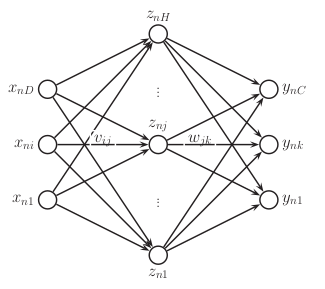
\includegraphics[width=.5\textwidth]{./chapters/3_classical_learning/01_supervised_learning/3_images/1_neural_network_one_hl.png}
    \end{center}
    \caption{caption}
    \label{fig:1_neural_network_one_hl}
\end{figure}
\subparagraph{Convolutional Neural Networks}
It is an MLP in which \tB{the hidden units have local receptive fields}, and in which \tB{the weights
are \emph{tied} or \emph{shared} across the image in order to reduce the number of parameters}. 
Intuitively the \tB{effect of such spatial parameter tying is that any useful features that are 
"discovered" in some portion of the image can be re-used everywhere else without having to be
independently learned}. The resulting network then exhibits \emph{translation invariance} meaning
it can classify patterns no matter where they occur inside the input image.

\paragraph{Strengths}
\paragraph{Weaknesses}
\paragraph{Relationships with other methods}
\paragraph{Examples of application}


%\subsection{Logistic Regression}
%\paragraph{Purpose}
%\paragraph{Assumptions}
%\paragraph{Theory}
%\paragraph{Strengths}
%\paragraph{Weaknesses}
%\paragraph{Relationships with other methods}
%\paragraph{Examples of application}


\section{Model Selection}
\subsection{Bayesian Variable Selection}
\paragraph{Purpose}
Let \tB{$\gamma_{j}: 
\begin{cases}
    \gamma_{j} = 1 \Leftarrow \text{feature } j \text{ is relevant}\\
    \gamma_{j} = 0 \Leftarrow \text{otherwise}\\
\end{cases}$} our goal is to compute the posterior over models:
\begin{center}
    $\prob{\gamma|\mathcal{D}} = \dfrac{e^{-f(\gamma)}}{\su{\gamma'}{}e^{-f(\gamma')}}$
\end{center}
where the cost function is defined by $f(\gamma) \triangleq -\left[\log\left(\prob{
\mathcal{D}|\gamma}\right) + \log\left(\prob{\gamma}\right)\right]$

\paragraph{Assumptions}
\paragraph{Theory}
\subparagraph{Spike and slab model}
remember that posterior is given by $\prob{\bm{\gamma}|\mathcal{D}}\propto \prob{
\mathcal{D}|\bm{\gamma}}\prob{\bm{\gamma}}$.\\
It is common to use the following prior $\prob{\bm{\gamma}} = \prd{j=1}{D}\text{
\emph{Ber}}(\gamma_{j}|\pi_{0}) = \pi_{0}^{\norm{\gamma}_{0}}(1-\pi_{0})^{D-\norm{
\gamma}_{0}}$, where $\pi_{0}$ is the probability that a feature is relevant.\\
The likelihood is defined as follows: $\prob{\mathcal{D}|\bm{X},\bm{\gamma}} = 
\Su{}{}\Su{}{}\prob{\bm{y}|\bm{X},\bm{w},\bm{\gamma}}\prob{\bm{w}|\bm{\gamma},
\sigma^{2}}\prob{\sigma^{2}}d\bm{w}d\sigma^{2}$\\
Consider the prior $\prob{\bm{w}|\bm{\gamma},\sigma^{2}}$ in standardizing the inputs, 
a reasonable prior is $\mathcal{N}(0, \sigma^{2}\sigma_{w}^{2})$, where 
$\sigma_{w}^{2}$ controls how big we expect the coefficients associated with the 
relevant variables to be, which is scaled by the overall noise. We can summarize this 
prior as follows: $\prob{\bm{w}_{j}|\sigma^{2},\gamma_{j}}
\begin{cases}
    \delta_{0}(w_{j}) \Leftarrow \gamma_{j} = 0\\
    \mathcal{N}(w_{j}|0, \sigma^{2}\sigma_{w}^{2}) \Leftarrow \gamma_{j} = 1
\end{cases}$
\uB{the first term is a "spike" at the origin, as $\sigma_{w}^{2}\rightarrow +\infty$ 
the distribution $\prob{w_{j}|\gamma_{j} = 1}$ approaches a uniform distribution which 
can be thought of as a "slab"}.

\subparagraph{Bernoulli-Gaussian model}
we have 
$\begin{cases}
    \prob{y_{i}|\bm{x}_{i},\bm{w}, \bm{\gamma},\sigma^{2}} = \mathcal{N}\left(\su{j}{}
    \gamma_{j}w_{j}x_{ij}, \sigma^{2}\right) \\
    \prob{\gamma_{j}} = \text{\emph{Ber}}(\pi_{0})\\
    \prob{w_{j}} = \mathcal{N}(0, \sigma_{w}^{2})
\end{cases}$
we can think of the \tB{$\gamma_{j}$ as a masking out the weights $w_{j}$}. Unlike the
spike and slab model we do not integrate the irrelevant coefficients, they always 
exists.\\
\uB{One interesting aspect of this model is that it can be used to derive objective 
function that is widely used in the non-Bayesian subset selection literature.}
\subparagraph{Algorithms}
assuming that we want to find the MAP model.
\begin{itemize}
    \item Single best replacement: at each step, we define a \uB{neighborhood of the 
        current model to be all models than can be reached by flipping a single bit
        of $\gamma$}
    \item Orthogonal least squares: we start from an empty set of variables and we 
        add the best feature \tB{$j^{*} = \displaystyle\argmin_{j\notin\bm{\gamma}_{t}}\displaystyle
            \min_{\bm{w}}\norm{\bm{y}-\bm{X}_{\bm{\gamma}_{t}\cup j}\bm{w}}^{2}$} 
    \item Orthogonal matching pursuits: as Orthogonal least squares is somewhat 
        expensive, a simplification is to freeze the current weight and then pick the 
        next feature to add by solving \tB{$j^{*} = \displaystyle\argmin_{j\notin\bm{\gamma}_{t}}
        \displaystyle\min_{\beta} \norm{\bm{y}-\bm{X}\bm{w}_{t} - \beta\bm{x}_{\cdot j}}^{2}$}. And
        $\beta = \dfrac{\bm{x}_{\cdot j}^{T}\bm{r}_{t}}{\norm{\bm{x}_{\cdot j}}^{2}}$, where
        $\bm{r} = \bm{y}-\bm{X}\bm{w}_{t}$
    \item Backward selection: starts with all variables in the model and deletes the
    \item Bayesian matching pursuits: similar to OMP except it uses a Bayesian marginal
        likelihood scoring criterion instead of a least square objective.
\end{itemize}

\paragraph{Strengths}
\paragraph{Weaknesses}
\paragraph{Relationships with other methods}
\paragraph{Examples of application}


\subsection{Least Angle Regression Shrinkage}
\paragraph{Purpose}
Instead of updating only one variable at a time, inducing slow converging, we can use \uB{\emph{
Active set} methods that update many variables at a time}. They add or remove a few variables at
a time so they can take a long time if they started far from the solution.\\
Suppose $\mathcal{A}_{k}$ is the active set of variables at the 
beginning of the $k^{th}$ step and let $\beta_{\mathcal{A}_{k}}$ be the
coefficient vector for these variables at this step, there will be 
$k-1$ nonzero values and the one just entered will be zero.\\
If \uB{$\bm{r}_{k}=\bm{y}-\bm{X}_{\mathcal{A}_{k}}\beta_{\mathcal{A}_{k}}$}
is the current residual, then the direction for this step is:
\begin{center}
    $\delta_{k}=(\bm{X}_{\mathcal{A}_{k}}^{T}\bm{X}_{\mathcal{A}_{k}})^{-1}\bm{X}_{\mathcal{A}_{k}^{T}}^{T}\bm{r}_{k}$
\end{center}
The name ``least angle'' arises from a geometrical interpretation of 
this process; $\bm{u}_{k}$ makes the smallest (and equal) angle with
each of the predictors in $\mathcal{A}_{k}$
\paragraph{Assumptions}
\paragraph{Theory}
Active methods exploit the fact that one can quickly compute $\hat{\bm{w}}(\lambda_{k})$ from 
$\hat{\lambda}(\lambda_{k-1})$ if $\lambda_{k}\approx\lambda_{k-1}$ this is known as \textbf{warm
starting}.

\subparagraph{Least Angle Regression}
\begin{enumerate}
	\item \uB{Standardize the predictors} to have mean zero an unit 
		norm.\\ \uB{Start with the residual $\bm{r}=\bm{y}-
		\overline{\bm{y}}$}, and for all $j\in\inter{1}{p},~\beta_{j}=0$
    \item Find the predictor $x_{j}$ most correlated with $\bm{r}$
    \item For $j\in\inter{1}{p}$
    \begin{itemize}
        \item Move $\beta_{j}$ from 0 to its least-squares coefficient
            $\dfrac{\sP{\bm{x}_{j}}{\bm{r}}}{\sP{\bm{x}_{j}}{\bm{x}_{j}}}$, then recompute 
            $\bm{r}$. Find the predictor $x_{k}$ most correlated with the new $\bm{r}$
        \item Move $\beta_{k}$ from 0 to its least-squares coefficient
            $\dfrac{\sP{\bm{x}_{k}}{\bm{r}}}{\sP{\bm{x}_{k}}{\bm{x}_{k}}}$, then recompute 
            $\bm{r}$. Find the predictor $x_{l}$ most correlated with the new $\bm{r}$\dots
        \item Move $\beta_{j}$ and $\beta_{k}$ in the direction defined
            by their joint least squares coefficient of the current
            residual on $(x_{j},x_{k})$, until some other 
            competitor $x_{l}$ has as much correlation with the
            current residual.
    \end{itemize}
	\item After $\min(N-1, p)$ steps, we arrive at the
		full least-squares solution.
\end{enumerate}

\subparagraph{Least Angle Regression: Lasso Modification}
\begin{itemize}
	\item[4a] If a non-zero coefficient hits zero, drop its variable from the
		active set of varibalbes and recompute the current joint least squares
		direction
\end{itemize}


\paragraph{Strengths}
\begin{itemize}
	\item Numerically efficient when $p\gg n$
	\item As fast as forward selection and has the same order of complexity as OLS
	\item Produces a full piecewise linear solution path
	\item Stable
	\item Esealy modified to produce for other estimators like the Lasso
\end{itemize}

\paragraph{Weaknesses}
\begin{itemize}
    \item Because LARS is based upon iterative refitting of the residuals, it would
		appears to be especially sensitive to the effect noise.
\end{itemize}

\paragraph{Relationships with other methods}
\begin{itemize}
    \item Least Squares
\end{itemize}

\paragraph{Examples of application}


%\subsection{Logistic Regression}
%\paragraph{Purpose}
%\paragraph{Assumptions}
%\paragraph{Theory}
%\paragraph{Strengths}
%\paragraph{Weaknesses}
%\paragraph{Relationships with other methods}
%\paragraph{Examples of application}


\section{Regularization}
\subsection{$l_{1}$ regularization}
\paragraph{Purpose}

\paragraph{Assumptions}
We assume $\prob{\bm{w}|\lambda} = \prd{j=1}{D}\text{\emph{Lap}}(w_{j}|0,
\frac{1}{\lambda}) \propto \prd{j=1}{D}e^{-\lambda|w_{j}|}$
\paragraph{Theory}
For penalized negative log likelihood has the form: $f(\bm{w}) = -\log\left(\prob{
\mathcal{D}|\bm{w}}\right) - \log\left(\prob{\bm{w}|\lambda}\right) = \text{\emph{NLL}}
(\bm{w}) + \lambda\norm{\bm{w}}_{1}$.\\
Geometrically we understand that as we relax the constraint we grow $l_{1}$ ball until
it meets the objective, \tB{the corners of the ball are more likely to intersect the
ellipse than one of the sides} especially in high dimensions because the corners "stick
out". The corners correspond to sparse solutions which lie on the coordinate axes. By
contrast when we grow the $l_{2}$ ball it can intersect the objective at any point, 
there are no "corners" so there is no preference for sparsity. 
\paragraph{Strengths}

\paragraph{Weaknesses}
\begin{itemize}
    \item can give quite different results if the data is slightly perturbed
\end{itemize}
\paragraph{Relationships with other methods}
\paragraph{Examples of application}

\subsection{Regularization path}
\paragraph{Purpose}
As we increase $\lambda$, the solution vector $\hat{\bm{w}}(\lambda)$ will tend to get
sparser, although not necessary monotonically. For each feature $j$ we can plot the 
values $\hat{w}_{j}(\lambda)$ vs $\lambda$ which is known as \emph{regularization path}
\paragraph{Assumptions}
\paragraph{Theory}
\paragraph{Strengths}
\paragraph{Weaknesses}
\paragraph{Relationships with other methods}
\paragraph{Examples of application}

\subsection{Coordinate Descent}
\paragraph{Purpose}
These algorithms exploit the fact that one can quickly compute $\hat{\bm{w}}(
\lambda_{k})$ from $\hat{\bm{w}}(\lambda_{k-1})$ if $\lambda_{k} \approx \lambda_{k-1}$
this is known as \emph{warm starting}.
\paragraph{Assumptions}
\paragraph{Theory}
\subparagraph{Coordinate descent}
$w^{*}_{j} = \argmin_{z}f(\bm{w} + z\bm{e}_{j}) - f(\bm{w})$ with $\bm{e}_{j}$ is the 
\emph{j}'th unit vector. 

\paragraph{Strengths}
\begin{itemize}
    \item if each one-dimensional optimization problem can be solved analitically
\end{itemize}

\paragraph{Weaknesses}
\paragraph{Relationships with other methods}
\paragraph{Examples of application}

%\subsection{Logistic Regression}
%\paragraph{Purpose}
%\paragraph{Assumptions}
%\paragraph{Theory}
%\paragraph{Strengths}
%\paragraph{Weaknesses}
%\paragraph{Relationships with other methods}
%\paragraph{Examples of application}

